\documentclass{article}

\usepackage{fullpage}



\usepackage[all=normal,bibliography=tight]{savetrees}

\usepackage{tikz}
\usetikzlibrary{snakes}
\usetikzlibrary{positioning}
\usetikzlibrary{decorations.markings}
\usepackage{xspace}
\usepackage{comment}

\usepackage{amsmath,amstext,amssymb,amsthm}

\newtheorem{theorem}{Theorem}[section]
\newtheorem{lemma}[theorem]{Lemma}
\newtheorem{definition}[theorem]{Definition}
\newtheorem{corollary}[theorem]{Corollary}
\newtheorem{remark}[theorem]{Remark}
\newtheorem{proposition}[theorem]{Proposition}

\theoremstyle{definition}
\newtheorem{example}[theorem]{Example}

\begin{document}

\newcommand{\schedname}{{\sc{SCHED}}\xspace}
\newcommand{\schedlongname}{\xspace}
\newcommand{\czas}[1]{t(#1)}
\newcommand{\koszt}[1]{T(#1)}
\newcommand{\tudu}[1]{{\bf{TODO: #1}}}
\newcommand{\eps}{\varepsilon}
\newcommand{\pinezka}{\textrm{nil}}
\newcommand{\pred}{{\ensuremath{pred}}}
\newcommand{\succc}{{\ensuremath{succ}}}
\renewcommand{\subset}{\subseteq}
\newcommand{\Oh}{\ensuremath{O}}
\newcommand{\Ohstar}{\ensuremath{\Oh^\ast}}

\newcommand{\Wvc}{M}
\newcommand{\Whalf}{W_{\mathrm{half}}}
\newcommand{\Wquarter}{W_{\mathrm{quarter}}}
\newcommand{\matching}{\mathcal{M}}

\newcommand{\defproblemnoparam}[3]{
  \vspace{1mm}
\noindent\fbox{
  \begin{minipage}{\textwidth}  
  #1 \\ 
  {\bf{Input:}} #2  \\
  {\bf{Task:}} #3
  \end{minipage}
  }
  \vspace{1mm}
}

\definecolor{light-gray}{gray}{0.8}

\title{Scheduling partially ordered jobs faster than \thanks{An extended abstract of this paper appears at 19th European Symposium on Algorithms, Saarbr\"{u}cken, Germany, 2011.}}

  \author{Marek Cygan\thanks{Institute of Informatics, University of Warsaw, Poland, \texttt{cygan@mimuw.edu.pl}. Supported by Polish Ministry of Science grant no. N206 355636 and Foundation for Polish Science.} \and
	Marcin Pilipczuk\thanks{Institute of Informatics, University of Warsaw, Poland, \texttt{malcin@mimuw.edu.pl}. Supported by Polish Ministry of Science grant no. N206 355636 and Foundation for Polish Science.} \and
	Micha\l{} Pilipczuk\thanks{Faculty of Mathematics, Informatics and Mechanics, University of Warsaw, Poland, \texttt{michal.pilipczuk@students.mimuw.edu.pl}} \and
	Jakub Onufry Wojtaszczyk\thanks{Google Inc., Cracow, Poland, \texttt{onufry@google.com}}}

\date{}

\maketitle

\begin{abstract}
In a scheduling problem, denoted by \schedlongname in the Graham notation,
we are given a set of  jobs, together with their processing
times and precedence constraints. The task is to order the jobs so that their total completion time is minimized.
\schedlongname is a special case of the Traveling Repairman Problem with precedences.
A natural dynamic programming algorithm solves both these problems in  time, and whether
there exists an algorithms solving \schedlongname{} in  time for some constant 
was an open problem posted in 2004 by Woeginger. In this paper we answer this question positively.
\end{abstract}

\section{Introduction}

It is commonly believed that no NP-hard problem is solvable in polynomial time.
However, while all NP-complete problems are equivalent with respect to polynomial time reductions,
they appear to be very different with respect to the best exponential time exact solutions.
In particular, most NP-complete problems can be solved significantly faster than
the (generic for the NP class) obvious brute-force algorithm that checks all possible solutions;
examples are {\sc Independent Set}~\cite{fgk:m-c-jacm}, {\sc Dominating Set}~\cite{fgk:m-c-jacm,rooij:domsetesa09}, {\sc Chromatic Number}~\cite{bjohus:color} and
{\sc Bandwidth}~\cite{nasz-tcs}.
The area of moderately exponential time algorithms studies upper and lower bounds
for exact solutions for hard problems.
The race for the fastest exact algorithm inspired several very interesting tools
and techniques such as Fast Subset Convolution~\cite{bjohus:fourier} and Measure\&Conquer~\cite{fgk:m-c-jacm}
(for an overview of the field we refer the reader to a recent book by Fomin and Kratsch~\cite{fomin-book}).

For several problems, including {\sc TSP}, {\sc Chromatic Number}, {\sc Permanent},
{\sc Set Cover}, {\sc \#Hamiltonian Cycles} and {\sc SAT}, the currently best known time complexity
is of the form\footnote{The  notation suppresses factors polynomial in the input size.}
, which is a result of applying dynamic programming over subsets,
the inclusion-exclusion principle or a brute force search.
The question remains, however, which of those problems are inherently so hard that it is
not possible to break the  barrier and which are just waiting for new tools and techniques still to be discovered.
In particular, the hardness of the -{\sc SAT} problem is the starting point for the
Strong Exponential Time Hypothesis of Impagliazzo and Paturi~\cite{seth},
which is used as an argument that other problems are hard~\cite{cut-and-count,treewidth-lower,patrascu}.
Recently, on the positive side,  time algorithms for a constant  have been developed for
{\sc Capacitated Domination}~\cite{capdomset}, {\sc Irredundance}~\cite{irrset},
{\sc Maximum Induced Planar Subgraph}~\cite{fomin-esa11} and
(a major breakthrough in the field)
for the undirected version of the {\sc Hamiltonian Cycle} problem~\cite{bjorklund-focs}.

In this paper we extend this list by one important scheduling problem.
The area of scheduling algorithms originates from practical questions regarding scheduling jobs on single- or multiple-processor
machines or scheduling I/O requests. It has quickly become one of the most important areas in algorithmics, with significant influence on other branches of computer science.
For example, the research of the job-shop scheduling problem in 1960s resulted
in designing the competitive analysis \cite{graham:jobshop}, initiating the research of
online algorithms.
Up to today, the scheduling literature consists of thousands of research publications.
We refer the reader to the classical textbook of Brucker \cite{sched:book}.

Among scheduling problems one may find a bunch of problems solvable in polynomial time, as well as many NP-hard ones.
For example, the aforementioned job-shop problem is NP-complete on at least three machines \cite{job-shop:3},
but polynomial on two machines with unitary processing times \cite{job-shop:2}.

Scheduling problems come in numerous variants. For example, one may consider
scheduling on one machine, or many uniform or non-uniform machines.
The jobs can have different attributes: they may arrive at different times,
may have deadlines or precedence constraints, preemption may or may not be allowed.
There are also many objective functions, for example the makespan of the computation,
total completion time, total lateness (in case of deadlines for jobs) etc.

Let us focus on the case of a single machine. Assume we are given a set of jobs ,
and each job  has its processing time .
For a job , its completion time is the total amount of time that this job waited
to be finished; formally, the completion time of a job  is defined as the sum
of processing times of  and all jobs scheduled earlier.
If we are to minimize the total completion time (i.e, the sum of completion times
over all jobs), it is clear that the jobs should be scheduled in order of increasing
processing times.
The question of minimizing the makespan of the computation (i.e., maximum completion time)
is obvious in this setting, but we note that minimizing makespan is polynomially solvable even
if we are given a precedence constraints on the jobs (i.e., a partial order on the set of jobs
is given, and a job cannot be scheduled before all its predecessors in the partial order
are finished) and jobs arrive at different times (i.e., each job has its arrival time,
  before which it cannot be scheduled) \cite{lawler:sched}.

Lenstra and Rinnooy Kan \cite{lenstra} in 1978 proved that
the question of minimizing total completion time on one machine becomes NP-complete
if we are given precedence constraints on the set of jobs.
To the best of our knowledge the currently smallest approximation ratio for this case equals ,
due to independently discovered algorithms by Chekuri and Motwani~\cite{chekuri} as well as Margot et al.~\cite{margot}.
The problem of minimizing total completion time on one machine, given
precedence constraints on the set of jobs, can be solved
by a standard dynamic programming algorithm in time , where  denotes the
number of jobs.
In this paper we break the -barrier for this problem.

Before we start, let us define formally the considered problem.
As we focus on a single scheduling problem, for brevity we
denote it by \schedname{}. We note that the proper name of this problem in the Graham notation
    is \schedlongname{}.

\defproblemnoparam{\schedname{}}
{A partially ordered set of jobs ,
together with a nonnegative processing time  for each job .
}
{
Compute a bijection  (called an {\em{ordering}})
that satisfies the precedence constraints (i.e., if , then )
and minimizes the total completion time of all jobs defined as

}

If  for  (i.e.,  and ),
we say that  {\em{precedes}} ,  is a {\em{predecessor}}
or {\em{prerequisite}} of ,  is {\em{required}} for  or that  is a {\em{successor}}
of . We denote  by .

\schedname{} is a special case of the precedence constrained Travelling Repairman Problem (prec-{\sc TRP}), defined as follows. A repairman needs to visit all vertices of a (directed
or undirected) graph  with distances  on edges.
At each vertex, the repairman is supposed to repair a broken machine;
a cost of a machine  is the time  that it waited before being repaired.
Thus, the goal is to minimize the total repair time, that is, .
Additionally, in the precedence constrained case, we are given a partial order 
on the set of vertices of ; a machine can be repaired only if all its predecessors
are already repaired.
Note that, given an instance  of \schedname{},
we may construct equivalent prec-{\sc{TRP}} instance, by taking  to be a complete directed
graph on the vertex set , keeping the precedence constraints unmodified, and setting
.

The {\sc{TRP}} problem is closely related to the Traveling Salesman Problem ({\sc{TSP}}).
All these problems are NP-complete and solvable in  time by
an easy application of the dynamic programming approach (here  stands for the number
of vertices in the input graph).
In 2010, Bj\"{o}rklund \cite{bjorklund-focs} discovered a genuine way to solve
probably the easiest NP-complete version of the {\sc{TSP}} problem --- the question
of deciding whether a given undirected graph is Hamiltonian --- in randomized
 time. However, his approach does not extend to directed graphs,
not even mentioning graphs with distances defined on edges.

Bj\"{o}rklund's approach is based on purely graph-theoretical and combinatorial reasonings,
and seem unable to cope with arbitrary (large, real) weights (distances, processing times).
This is also the case with many other combinatorial approaches.
Probably motivated by this,
Woeginger at International Workshop on Parameterized and Exact Computation
(IWPEC) in 2004~\cite{woeginger04} has posed the question (repeated in 2008~\cite{woeginger08}),
whether it is possible to construct an  time algorithm for the \schedname{} problem\footnote{Although Woeginger in his papers asks for an  algorithm, the intention is clearly to ask for an  algorithm.}.
This problem seems to be the easiest case of the aforementioned
family of {\sc{TSP}}-related problems with arbitrary weights.
In this paper we present such an algorithm, thus affirmatively answering Woeginger's question.
Woeginger also asked~\cite{woeginger04,woeginger08} whether an  time algorithm
for one of the problems {\sc TRP}, {\sc TSP}, prec-{\sc TRP}, \schedname{} implies 
time algorithms for the other problems. This problem is still open.

The most important ingredient of our algorithm is a combinatorial lemma (Lemma~\ref{lem:core})
which allows us to investigate the structure of the \schedname{} problem.
We heavily use the fact that we are solving the \schedname{} problem and
not its more general TSP related version, and for this reason
we believe that obtaining  time algorithms for other problems
listed by Woeginger is much harder.

\section{The algorithm}

\subsection{High-level overview --- part 1}\label{sec:high-level1}
Let us recall that our task in the \schedname{} problem is to compute an ordering 
that satisfies the precedence constraints (i.e., if  then )
and minimizes the total completion time of all jobs defined as

We define {\em{the cost of job  at position }} to be .
Thus, the total completion time is the total cost of all jobs at their respective
positions in the ordering .

We begin by describing the algorithm that solves \schedname in  time, which we call {\em{the DP algorithm}}
--- this will be the basis for our further work.
The idea --- a standard dynamic programming over subsets --- is that if we decide that a particular
set  will (in some order) form the prefix of our optimal , then the order
in which we take the elements of  does not affect the choices we make regarding the ordering
of the remaining ; the only thing that matters are the precedence constraints
imposed by  on . Thus, for each candidate set  to form a prefix,
the algorithm computes a bijection
 that minimizes the cost of jobs from , i.e.,
it minimizes .
The value of  is computed using the following easy to check recursive formula:

Here, by  we mean the set of maximum elements of  --- those which do not precede any element of .
The bijection  is constructed by prolonging  by ,
where  is the job at which the minimum is attained.
Notice that  is exactly the ordering we are looking for.
We calculate  recursively, using formula (\ref{eqn:reccost}),
storing all computed values  in memory to avoid recomputation.
Thus, as the computation of a single  value given all the smaller values
takes polynomial time, while  for each  is computed at most once
the whole algorithm indeed runs in  time.

The overall idea of our algorithm is to identify a family of sets  that --- for some
reason --- are not reasonable prefix candidates, and we can skip them in the computations of the
DP algorithm; we will call these {\em unfeasible sets}. If the number of feasible sets is not
larger than  for some , we will be done --- our recursion will visit only
feasible sets, assuming  to be  for unfeasible  in formula
(\ref{eqn:reccost}), and the running time will be . This is formalized
in the following proposition.

\begin{proposition}\label{prop:cut-dp}
Assume we are given a polynomial-time algorithm  that, given a set ,
either accepts it or rejects it. Moreover, assume that the number of sets accepted by 
is bounded by  for some constant . Then one can find in time  an optimal
ordering of the jobs in  among those orderings  where  is
accepted by  for all , whenever such ordering exists.
\end{proposition}
\begin{proof}
Consider the following recursive procedure to compute optimal  for a given set :
\begin{enumerate}
\item if  is rejected by , return ;
\item if , return ;
\item if  has been already computed, return the stored value of ;
\item otherwise, compute  using formula \eqref{eqn:reccost}, calling recursively the procedure
itself to obtain values  for , and store the computed value
for further use.
\end{enumerate}
Clearly, the above procedure, invoked on , computes optimal  among those orderings
 where  is accepted by  for all .
It is straightforward to augment this procedure to return the ordering  itself, instead of only its cost.

If we use balanced search tree to store the computed values of ,
each recursive call of the described procedure runs in polynomial time.
Note that the last step of the procedure is invoked at most once for each set  accepted by 
and never for a set  rejected by .
As an application of this step results in at most  recursive calls,
we obtain that a computation of  using this procedure results in the number
of recursive calls bounded by  times the number of sets accepted by . The time bound follows.
\end{proof}

\subsection{The large matching case}

We begin by noticing that the DP algorithm needs to compute  only for those
 that are downward closed, i.e., if  and  then .
If there are many constraints in our problem, this alone will suffice to limit the number
of feasible sets considerably, as follows.
Construct an undirected graph  with the vertex set  and edge set .
Let  be a maximum matching\footnote{Even an inclusion-maximal matching, which can be found greedily, is enough.}
in , which can be found in polynomial time \cite{mucha-sankowski:matching}.
If  is downward closed, and , , then it is not possible that  and .
Obviously checking if a subset is downward closed can be performed in polynomial time, thus we can apply Proposition \ref{prop:cut-dp},
accepting only downward closed subsets of .
This leads to the following lemma:
\begin{lemma}\label{lem:matching}
The number of downward closed subsets of  is bounded by .
If , then we can solve the \schedname problem in time
\qed
\end{lemma}
Note that for any small positive constant  the complexity  is of required order, i.e., 
 for some  that depends on .
Thus, we only have to deal with the case where .

Let us fix a maximum matching , let  be the set of endpoints of ,
and let .
Note that, as  is a maximum matching in , no two jobs in  are bound by a precedence constraint,
and , .
See Figure \ref{fig:matching} for an illustration.

\begin{figure}[htbp]
\begin{center}
\begin{tikzpicture}
    \tikzstyle{wvertex}=[circle,fill=black,minimum size=0.15cm,inner sep=0pt]
    \tikzstyle{ivertex}=[circle,draw=black,fill=light-gray,minimum size=0.15cm,inner sep=0pt]
    \centering
    \begin{scope}[shift={(0,-1.5)}]
      \draw[rounded corners=4pt] (-2, -1) rectangle (2,1) ;
      \draw (-2.5, 0) node {};
      \node[wvertex] (w1) at (-1.5,0) {};
      \node[wvertex] (w2) at (-0.5,-0.5) {};
      \node[wvertex] (w3) at (-0.5,0.5) {};
      \node[wvertex] (w4) at (0.5,-0.5) {};
      \node[wvertex] (w5) at (0.5,0.5) {};
      \node[wvertex] (w6) at (1.5, 0) {};
    \end{scope}
    \begin{scope}[shift={(0,1)}]
    \draw[rounded corners=4pt] (-5,-0.5) rectangle (5,0.5) ;
    \foreach \x in {1,2,...,19} {
      \node[ivertex] (a\x) at (-5 + \x*0.5, 0) {};
    }
    \draw (-5.5, 0) node {};
    \end{scope}
    \begin{scope}[decoration={markings,mark=at position 0.5 with {\arrow{>}}}]
      \foreach \a/\b in {w6/w4,w6/w5,w6/w2,w2/w1,w3/w1,w4/w3,w5/w3} {
        \draw[thick,postaction={decorate}] (\a) -- (\b);
      }
      \foreach \x in {1,2,...,7} {
        \draw[thick,postaction={decorate}] (-2+\x*0.25, -0.5) -- (-3+\x*0.25,0.5);
        \draw[thick,postaction={decorate}] (3-\x*0.25, 0.5) -- (2-\x*0.25,-0.5);
      }
    \end{scope}
\end{tikzpicture}
\caption{An illustration of the case left after Lemma \ref{lem:matching}.
In this and all further figures, an arrow points from the successor job to the predecessor one.}
\label{fig:matching}
\end{center}
\end{figure}



\subsection{High-level overview --- part 2}\label{sec:overview2}

We are left in the situation where there is a small number of ``special'' elements (),
and the bulk remainder (), consisting of elements that are tied by precedence constraints
only to  and not to each other.

First notice that if  was empty, the problem would be trivial: with no
precedence constraints we should simply order the tasks from the shortest to the longest.
Now let us consider what would happen if all the constraints between any  and
 would be of the form  --- that is, if the jobs from  had no predecessors.
For any prefix set candidate  we consider .
Now for any ,  we have an alternative prefix candidate:
the set . If , there has to be a reason
why  is not a strictly better prefix candidate than  --- namely, there has to exist
 such that , but .

A similar reasoning would hold even if not all of  had no predecessors, but just some
constant fraction  of  --- again, the only feasible prefix candidates would be those
in which for every  and  there is a reason (either
 or an element  which requires , but not ) not to exchange them.
It turns out that if , where , this observation suffices
to prove that the number of possible intersections of feasible sets with  is exponentially
smaller than . This is formalized and proved in
Lemma \ref{lem:core}, and is the cornerstone of the whole result.

A typical application of this lemma is as follows: say we have a set  of
cardinality , while
we know for some reason that all the predecessors of elements of  appear on positions
 and earlier. If  is large (a constant fraction of ), this is enough to limit
the number of feasible sets to . To this end it suffices
to show that there are exponentially
fewer than  possible intersections of a feasible set with . Each such intersection
consists of a set of at most  elements (that will be put on positions  through ),
and then a set in which every element has a reason not to be exchanged with something from
outside the set --- and there are relatively few of those by Lemma \ref{lem:core}
--- and when we do the calculations, it turns out the resulting number of
possibilities is exponentially smaller than .

To apply this reasoning, we need to be able to tell that all the prerequisites of a given
element appear at some position or earlier. To achieve this, we need to know the approximate
positions of the elements in . We achieve this by branching into  cases,
for each element  choosing to which of the four quarters of the set
 will  belong. This incurs a multiplicative cost\footnote{Actually, this bound can be improved to , as  are endpoints of a matching in the graph corresponding to the set of precedences.}
of ,
which will be offset by the gains from applying Lemma \ref{lem:core}.

We will now repeatedly apply Lemma \ref{lem:core} to obtain information about the
positions of various elements of . We will repeatedly say that if ``many'' elements
(by which we always mean more than  for some ) do not satisfy something,
we can bound the number of feasible sets, and thus finish the algorithm.
For instance, look at those elements of  which
can appear in the first quarter, i.e., none of their prerequisites appear in quarters
two, three and four. If there is more than  of them for some constant , we can apply the above
reasoning for  (Lemma \ref{lem:quarters1}).
Subsequent lemmata bound the number of feasible sets if there are many
elements that cannot appear in any of the two first quarters (Lemma \ref{lem:half}),
if {\em less} than  elements can appear in the first
quarter (Lemma \ref{lem:quarters1}) and if a constant fraction of elements
in the second quarter could actually appear in the first quarter
(Lemma \ref{lem:quarters2}). We also apply similar reasoning to elements that
can or cannot appear in the last quarter.

We end up in a situation where we have four groups of elements, each of size
roughly , split upon whether they can appear in the first quarter
and whether they can appear in the last one; moreover, those that can appear in
the first quarter will not appear in the second, and those that can appear in
the fourth will not appear in the third. This means that there are two pairs of parts
which do not interact, as the set of places in which they can appear are
disjoint. We use this independence of sorts to construct a different algorithm
than the DP we used so far, which solves our problem in this specific case
in time  (Lemma \ref{lem:finish-him}).

As can be gathered from this overview, there are many technical details we
will have to navigate in the algorithm. This is made more precarious by
the need to carefully select all the epsilons. We decided to use symbolic values for
them in the main proof, describing their relationship appropriately, using four constants
, . The constants  are very small positive reals, and additionally 
is much smaller than  for . At each step, we shortly discuss the existence
of such constants. We discuss the choice of optimal values of these constants in Section \ref{sec:values},
although the value we perceive in our algorithm lies rather in the existence
of an  algorithm than in the value of  (which is admittedly very small).

\subsection{Technical preliminaries}\label{sec:init}
We start with a few simplifications.
First, we add a few dummy jobs with no precedence constraints and zero processing times, so that  is divisible by four.
Second, by slightly perturbing the jobs' processing times, we can assume
that all processing times are pairwise different and, moreover, each ordering has different total completion time.
This can be done, for instance, by replacing time  with a pair ,
where  is an arbitrary numbering of . The addition of pairs is performed coordinatewise,
whereas comparison is performed lexicographically.
Note that this in particular implies that the optimal solution is unique, we denote it by .
Third, at the cost of an  multiplicative overhead,
we guess the jobs  and 
and we add precedence constraints  for each .
If  or  were not in  to begin with, we add them there.

A number of times our algorithm branches into several subcases, in each branch assuming some property
of the optimal solution . Formally speaking, in each branch we seek the optimal ordering
among those that satisfy the assumed property. We somewhat abuse the notation and denote by 
the optimal solution in the currently considered subcase.
Note that  is always unique within any subcase, as each ordering
has different total completion time.

For  by  we denote the set 
of predecessors of ,
and by  we denote the set  of successors of .
We extend this notation to subsets of : 
and .
Note that for any set , both  and  are subsets of .

In a few places in this paper we use the following simple bound on binomial coefficients
that can be easily proven using the Stirling's formula.
\begin{lemma}\label{lem:binom}
Let  be a constant. Then

In particular, if  then there exists a constant 
that depends only on  and

\end{lemma}

\subsection{The core lemma}\label{sec:core}

We now formalize the idea of exchanges presented at the beginning of Section \ref{sec:overview2}.
\begin{definition}\label{def:xch}
Consider some set , and its subset .
If there exists  such that for every  we can
find  with  then
we say  is {\em -exchangeable} with respect to , otherwise
we say  is {\em non--exchangeable} with respect to .

Similarly, if there exists  such that for every 
we can find  with ,
we call  {\em -exchangeable} with respect to , otherwise we call
it {\em non--exchangeable} with respect to .
\end{definition}

Whenever it is clear from the context, we omit the set  with respect to which its subset is
or is not - or -exchangeable.

Let us now give some more intuition on the exchangeable sets.
Let  be a non--exchangeable set with respect to  and let .
By the definition, there exists , such that for all 
we have ; in other words, all predecessors of  in  that are scheduled after 
have larger processing time than  --- which seems like a ``correct'' choice if we are to optimize the total completion time.

On the other hand, let  for some  and
assume that  is a -exchangeable set with respect to  with a job  witnessing this fact.
Let  be the job in  that is scheduled first in the optimal ordering .
By the definition, there exists  with .
It is tempting to decrease the total completion time of  by swapping the jobs  and  in : by the choice of , no precedence constraint
involving  will be violated by such an exchange, so we need to care only about the predecessors of .

We formalize the aforementioned applicability of the definition of - and -exchangeable sets in the following lemma:
\begin{lemma}\label{lem:exchange}
Let .
If for all  we have that , then for any  the set 
is non--exchangeable with respect to .

Similarly, if for all  we have ,
then the sets  are non--exchangeable with respect to .
\end{lemma}

\begin{proof}
The proofs for the first and the second case are analogous. However, to help the reader get intuition on exchangeable sets, we provide them both in full detail.
See Figure \ref{rysunek} for an illustration on the -exchangeable case.

{\underline{Non--exchangeable sets.}} Assume, by contradiction, that for some  the set  is -exchangeable.
Let  be a job witnessing it. Let  be the successor of  with minimum  (there exists one, as ). 
By Definition \ref{def:xch}, we have  with .
As , we have . As , we have .

Consider an ordering  defined as ,  and  if ;
in other words, we swap the positions of  and  in the ordering . We claim that  satisfies all the precedence constraints.
As ,  may only violates constraints of the form  and . However, if , then 
and  by the assumptions of the Lemma.
If , then , by the choice of .
Thus  is a feasible solution to the considered \schedname{} instance. Since , we have , a contradiction.

{\underline{Non--exchangeable sets.}} Assume, by contradiction, that for some  the set  is -exchangeable.
Let  be a job witnessing it. Let  be the predecessor of  with maximum 
(there exists one, as ). 
By Definition \ref{def:xch}, we have  with .
As , we have . As , we have .

Consider an ordering  defined as ,  and  if ;
in other words, we swap the positions of  and  in the ordering . We claim that  satisfies all the precedence constraints.
As ,  may only violates constraints of the form  and . However, if , then 
and  by the assumptions of the Lemma.
If , then , by the choice of .
Thus  is a feasible solution to the considered \schedname{} instance. Since , we have , a contradiction.
\end{proof}

\begin{figure}[htbp]
\begin{center}
\begin{tikzpicture}[scale=0.53]
    \centering
    \draw (-10.0,0.3) rectangle (10.0,-0.3);
    \draw (1.0,0.3) -- (1.0,-0.3);
    \draw (0.8,2.0) node {};
    \path[->] (0.8,1.5) edge (0.8,0.5);
\foreach \x in {-5,-4.5,-3.5,-2.0,-0.5,0.0,0.5,1.5,2.0,3.0,4.8,5.2,6.9,7.7,9.0}
	{
		\fill[light-gray] (\x,0) circle (0.15);
	}

    \foreach \x in {-9.75,-9,-8,-6.8,-5.5,-2.7,0.0,-1.2,2.5,4.0,6.0,8.2,9.8}
	{
		\fill[black] (\x,0) circle (0.15);
	}
    \foreach \x in {-9.75, -8, -6.8} {
		\fill[black] (\x-0.15, -0.15) rectangle (\x+0.15,0.15);
    }
    \foreach \x in {-5,-4.5,-3.5,-2.0,-0.5,0.0,0.5}
	{
		\draw[thick] (\x,0) circle (0.15);
	}

    \draw (-2.0,2.0) node {};
    \path[->] (-2.0,1.5) edge (-2.0,0.5);

    \draw (6.0,2.0) node {};
    \path[->] (6.0,1.5) edge (6.0,0.5);

    \draw (5.8,-0.3) -- (5.8,-0.8);
    \path[->] (5.8,-0.8) edge (10,-0.8);
    \draw (7.7, -1.3) node {};
    \draw (-6.6,-0.3) -- (-6.6,-0.8);
    \path[->] (-6.6,-0.8) edge (-10,-0.8);
    \draw (-8.1, -1.3) node {};

    \draw (3.0,2.0) node {};
    \path[->] (3.0,1.5) edge (3.0,0.5);

    \draw (-9.8,2.0) node {};
    \path[->] (-9.8,1.5) edge (-9.8,0.5);
    \draw (9.8,2.0) node {};
    \path[->] (9.8,1.5) edge (9.8,0.5);

    \path[<->] (-1.9,-0.4) edge [out=315, in=225] (2.9,-0.4);
\end{tikzpicture}
\caption{Figure illustrating the -exchangeable case of Lemma \ref{lem:exchange}. Gray circles indicate positions of elements of , black contour indicates that an element is also in . Black squares indicate positions of elements from , and black circles --- positions of other elements from .}
\label{rysunek}
\end{center}
\end{figure}

Lemma \ref{lem:exchange}
means that if we manage to identify a set  satisfying the assumptions
of the lemma, the only sets the DP algorithm has to consider are the
non-exchangeable ones. The following core lemma proves that there are few of
those (provided that  is big enough), and we can identify them easily.

\begin{lemma} \label{lem:core}
For any set  the number of non--exchangeable (non--exchangeable) subsets with regard to  is at most .
Moreover, there exists an algorithm
which checks whether a set is -exchangeable (-exchangeable) in polynomial
time.
\end{lemma}

The idea of the proof is to construct a function  that encodes each non-exchangeable set
by a subset of  no larger than .
To show this encoding is injective, we provide a decoding function  and show that
 is an identity on non-exchangeable sets.

\begin{proof}
As in Lemma \ref{lem:exchange}, the proofs for - and -exchangeable sets are analogous,
but for the sake or clarity we include both proofs in full detail.

{\underline{Non--exchangeable sets.}} 
For any set  we define the function 
 as follows:
for any element  we define  
(the {\em least expensive predecessor of}  {\em outside} ) to be the element of
 which has the smallest processing time,
or  if  is empty.
We now take  (the set of the {\em least expensive predecessors outside })
to be the set .
We see that  is indeed a set of cardinality at most .

Now we aim to prove that
 is injective on the family of non--exchangeable sets.
To this end we define the reverse function . For a set 
(which we think of as the set of the least expensive predecessors outside some )
let  be the set of such elements  of 
that there exists  such that for any  we have
. 
Notice, in particular, that , as for  and  we have .

First we prove  for any .
Take any  and consider any .
Then   and ,
as .
Thus , as for any  we can take a witness 
in the definition of .

In the other direction, let us assume that  does not satisfy .
This means we have .
Then we show that  is -exchangeable.
Consider any .
As , by the definition of the function  applied to the set ,
there exists  with
. But , while ;
and as all the values of  are distinct, 
and  satisfies the condition for  in the definition of
-exchangeability.

{\underline{Non--exchangeable sets.}}
For any set  we define the function 
 as follows:
for any element  we define  
(the {\em most expensive successor of}  {\em in} ) to be the element of
 which has the largest processing time,
or  if  is empty.
We now take  (the set of the {\em most expensive successors in })
to be the set .
We see that  is indeed a set of cardinality at most .

Now we aim to prove that  is injective on the family of non--exchangeable sets.
To this end we define the reverse function . For a set 
(which we think of as the set of most expensive successors in some )
let  be the set of such elements  of 
that for any  there exists a  with
. 
Notice, in particular, that , as for  the job  is a good witness for any .

First we prove  for any .
Take any  and consider any .
Then   and ,
as .
Thus , as for any  we can take 
in the definition of .

In the other direction, let us assume that  does not satisfy .
This means we have .
Then we show that  is -exchangeable.
Consider any .
As , by the definition of the function  applied to the set ,
 there exists  with
. But , while ;
and as all the values of  are distinct, 
and  satisfies the condition for  in the definition of
-exchangeability.

Thus, in both cases, if  is non-exchangeable then  (in fact it is possible
to prove in both cases that  is non-exchangeable iff ).
As there are  possible values of ,
the first part of the lemma is proven.
For the second, it suffices to notice that - and -exchangeability can be checked
in time  directly from the definition. 
\end{proof}

\begin{example}
To illustrate the applicability of Lemma \ref{lem:core}, we analyze the following very simple case:
assume the whole set  succeeds , i.e., for every  and  we have .
If  is small, then we can use the first case of Lemma \ref{lem:exchange} for the whole set : we have  and we
only look for orderings that put  as the first processed job.
Thus, we can apply Proposition \ref{prop:cut-dp} with algorithm  that rejects sets  where  is -exchangeable with respect to
. By Lemma \ref{lem:core}, the number of sets accepted by  is bounded by ,
which is small if .
\end{example}

\subsection{Important jobs at }\label{sec:half}

As was already mentioned in the overview, the assumptions of Lemma \ref{lem:exchange} are quite strict; therefore, we need to learn a bit more on how  behaves on  in order to distinguish a suitable place for an application. As , we can afford branching into few subcases for every job in .

Let , , , , i.e., we split  into quarters.
For each  we branch into two cases: whether  belongs to  or ;
however, if some predecessor (successor) of  has been already assigned to  (), we do not allow  to be placed in  ().
Of course, we already know that  and .
Recall that the vertices of  can be paired into a matching; since for each ,  we cannot have  placed in 
and  placed in , this branching leads to  subcases, and thus the same overhead in the time complexity.
By the above procedure, in all branches the guesses about alignment of jobs from  satisfy precedence constraints inside .

Now consider a fixed branch. 
Let  and  be the sets of elements of  to be placed in  and , respectively.


\begin{figure}[htbp]
\begin{center}
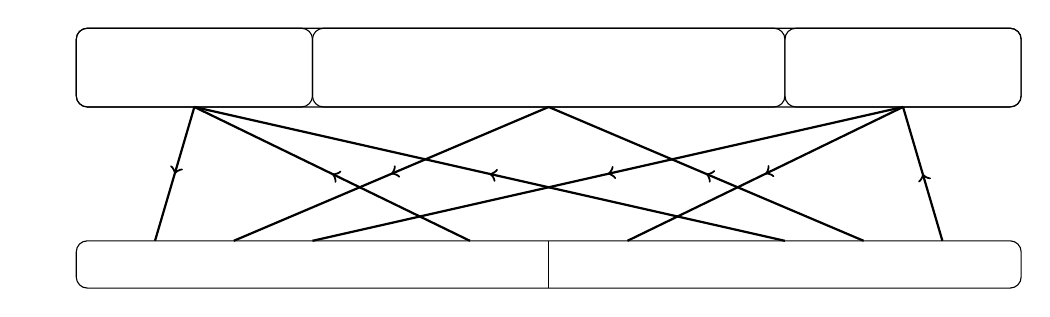
\begin{tikzpicture}
    \centering
\begin{scope}[shift={(0,-1)}]
      \draw[rounded corners=4pt] (-6, -0.3) rectangle (6,0.3) ;
      \draw (0,-0.3) -- (0,0.3);
      \draw (-3, 0) node {};
      \draw (3, 0) node {};
      \coordinate (MAB1) at (-5,0.3);
      \coordinate (MAB2) at (-4,0.3);
      \coordinate (MAB3) at (-3,0.3);
      \coordinate (MAB4) at (-1,0.3);
      \coordinate (MCD1) at (5,0.3);
      \coordinate (MCD2) at (4,0.3);
      \coordinate (MCD3) at (3,0.3);
      \coordinate (MCD4) at (1,0.3);
      \draw (-6.5,0) node {};
    \end{scope}
    \begin{scope}[shift={(0,2)}]
    \draw[rounded corners=4pt] (-6,-1) rectangle (6,0);
    \draw[rounded corners=4pt] (-6,-1) rectangle (-3,0);
    \draw[rounded corners=4pt] (3,-1) rectangle (6,0);
    \draw[rounded corners=4pt] (-3,-1) rectangle (3,0);
    \coordinate (WAB) at (-4.5,-1);
    \coordinate (WCD) at (4.5,-1);
    \coordinate (I2) at (0,-1);
    \draw (-4.5,-0.5) node {};
    \draw (4.5,-0.5) node {};
    \draw (0,-0.5) node {};
    \draw (-6.5,-0.5) node {};
    \end{scope}
    \begin{scope}[decoration={markings,mark=at position 0.5 with {\arrow{>}}}]
      \foreach \a/\b in {MAB1/WAB, MAB2/I2, MAB3/WCD, WAB/MAB4, WAB/MCD3, MCD4/WCD, I2/MCD2, WCD/MCD1} {
        \draw[thick,postaction={decorate}] (\b) -- (\a);
      }
    \end{scope}
\end{tikzpicture}
\caption{An illustration of the sets , ,  and .}
\label{fig:half}
\end{center}
\end{figure}

Let us now see what we can learn in a fixed branch about the behaviour of  on .
Let 

that is  (resp. ) are those elements of  which are forced into the first (resp. second) half of 
by the choices we made about  (see Figure \ref{fig:half} for an illustration).
If one of the  sets is much larger than , we have obtained a gain --- by branching into at most  branches we gained
additional information about a significant (much larger than ) number of other elements (and so we will be able to avoid considering a significant number of
sets in the DP algorithm).
This is formalized in the following lemma:

\begin{lemma}\label{lem:half}
Consider a fixed branch.
If  or  has at least  elements, then the DP algorithm can be augmented to solve the instance in the considered branch in time

\end{lemma}

\begin{proof}
We describe here only the case . The second case is symmetrical.

Recall that the set  needs to be placed in  by the optimal ordering .
We use Proposition \ref{prop:cut-dp} with an algorithm  that accepts sets 
such that the set  (the elements of  not scheduled in ) is of size at most  (the number
of jobs to be scheduled after  in the first half of the jobs).
Moreover, the algorithm  tests if the set  conforms with the guessed sets  and , i.e.:

Clearly, for any , the set  is accepted by ,
as  places  in  and  in .

Let us now estimate the number of sets  accepted by . Any set  of size larger than  needs to contain ; there are
at most  such sets. All sets of size at most  are accepted by ; there
are at most  such sets. 
Consider now a set  of size  for some . Such a set needs to contain
 elements of  for some  and  elements of .
Therefore the number of such sets (for all possible ) is bounded by:

The last inequality follows from the fact that the function  is decreasing for .
The bound  follows.


\end{proof}

Note that we have  overhead so far, due to guessing placement of the jobs from .
By Lemma \ref{lem:binom},  and ,
for some positive constants  and  that depend only on .
Thus, for any small fixed  we can choose  sufficiently small
so that  for some . Note that  is an upper bound on the total time spent on processing all the considered subcases.

Let  and . From this point we assume that , hence 
and .
For each  we branch into two subcases, whether  belongs to  or . Similarly, for each 
we guess whether 
belongs to  or . Moreover, we terminate branches which are trivially contradicting the constraints.

Let us now estimate the number of subcases created by this branch.
Recall that the vertices of  can be paired into a matching; since for each ,  we cannot have  placed in a later segment than ;
this gives us  options for each pair .
Thus, in total they are at most  ways of placing vertices of  into quarters without contradicting the constraints.
Moreover, this step gives us an additional  overhead in the time complexity for vertices in .
Overall, at this point we are considering at most  subcases.

We denote the set of elements of  and  assigned to quarter  by  and , respectively.

\subsection{Quarters and applications of the core lemma}\label{sec:appl-core}

In this section we try to apply Lemma \ref{lem:core} as follows:
We look which elements of  can be placed in  (the set ) and which cannot (the set ).
Similarly we define the set  (can be placed in ) and  (cannot be placed in ).
For each of these sets, we try to apply Lemma \ref{lem:core} to some subset of it.
If we fail, then in the next subsection we infer that the solutions in the quarters are partially independent of
each other, and we can solve the problem in time roughly .
Let us now proceed with a more detailed argumentation.

We define the following two partitions of :

In other words, the elements of  cannot be placed in  because some of their requirements are in ,
   and the elements of  cannot be placed in  because they are required by some elements of  (see Figure \ref{fig:PA} for an illustration).
 Note that these definitions are independent of , so sets  for  can be computed in polynomial time. Let 


\begin{figure}[htbp]
\begin{center}
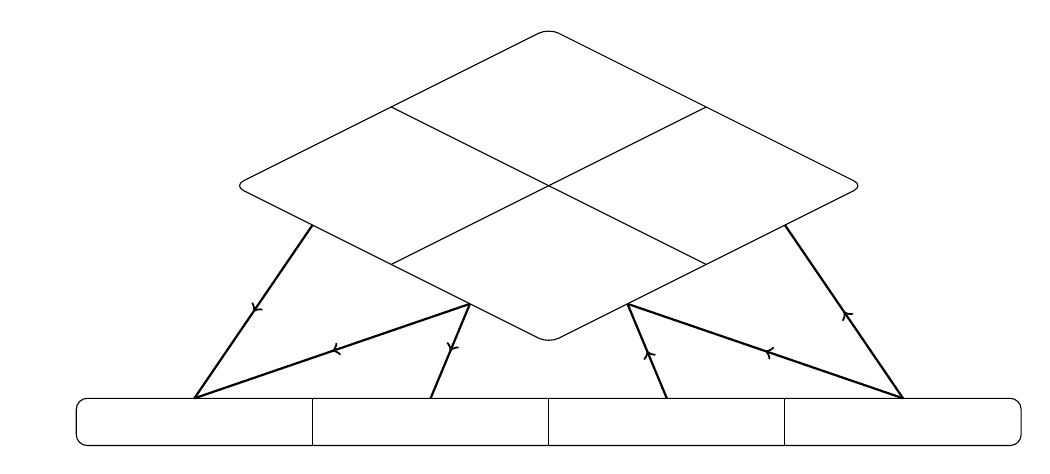
\begin{tikzpicture}
    \centering
\begin{scope}[shift={(0,-1)}]
      \draw[rounded corners=4pt] (-6, -0.3) rectangle (6,0.3) ;
      \foreach \x/\n in {1/A,2/B,3/C,4/D} {
        \draw (-7.5 + \x*3, 0) node {};
        \coordinate (M\n) at (-7.5 + \x*3, 0.3);
      }
      \foreach \x in {1,2,3} {
        \draw (-6+\x*3,-0.3) -- (-6+\x*3,0.3);
      }
      \draw (-6.5,0) node {};
    \end{scope}
    \begin{scope}[shift={(0,2)},yscale=0.5]
    \draw[rounded corners=4pt] (-2,-2) -- (-4,0) -- (0, 4) -- (4, 0) -- (0, -4) -- (-2,-2);
    \draw (-2,-2) -- (2,2);
    \draw (2,-2) -- (-2,2);
    \coordinate (PA) at (-3,-1);
    \coordinate (PnA) at (-1,-3);
    \coordinate (PD) at (3,-1);
    \coordinate (PnD) at (1,-3);
    \draw (1.35,3.4) node {};
    \draw (3.35,1.4) node {};
    \draw (-1.35,3.35) node {};
    \draw (-3.35,1.35) node {};
    \draw (-4.5,0) node {};
    \end{scope}
    \begin{scope}[decoration={markings,mark=at position 0.5 with {\arrow{>}}}]
      \foreach \a/\b in {MA/PA, MA/PnA, MB/PnA, PD/MD, PnD/MD, PnD/MC} {
        \draw[thick,postaction={decorate}] (\b) -- (\a);
      }
    \end{scope}
\end{tikzpicture}
\caption{An illustration of the sets  for  and their relation
  with the sets  for .}
\label{fig:PA}
\end{center}
\end{figure}

Note that  for every .
As , , these values can be computed by the algorithm.
We branch into  further subcases, guessing the (still unknown) values  and .

Let us focus on the quarter  and assume that  is significantly smaller than  (i.e.,  is a constant fraction of ).
We claim that we can apply Lemma \ref{lem:core} as follows.
While computing , if , we can represent  as a disjoint sum of two subsets . The first one
is of size , and represents the elements of  placed in quarter , and the second represents the elements
of  placed in quarters . Note that the elements of  have all predecessors in the quarter , so by Lemma \ref{lem:exchange} the set  has to be non--exchangeable with respect to ; therefore, by Lemma \ref{lem:core}, we can consider only a very narrow choice of
. Thus, the whole part  can be represented by its subset of cardinality at most  plus some small information about the rest. If  is significantly smaller than , this representation is more concise than simply remembering a subset of . Thus we obtain a better bound on the number of feasible sets.

A symmetric situation arises when  is significantly smaller than ; moreover, we can similarly use Lemma \ref{lem:core} if  is significantly smaller than  or  than . This is formalized by the following lemma.
\begin{lemma}\label{lem:quarters0}
If  for some   and ,
then the DP algorithm can be augmented to solve the remaining instance in time bounded by

\end{lemma}

\begin{figure}[htbp]
\begin{center}
\begin{tikzpicture}
    \centering
    \begin{scope}[shift={(0,-2)}]
    \fill[light-gray] (-6,-0.3) rectangle (4,0.3);
    \foreach \x/\n in {1/A,2/B,3/C,4/D} {
      \draw (-9 + \x*3, -0.3) rectangle (-6+\x*3,0.3);
      \draw (-7.5 + \x*3,0) node {};
    }
    \foreach \x in {1,2,...,5} {
      \coordinate (A\x) at (-6+\x*0.5,0.35);
    }
    \foreach \x in {1,2,...,13} {
      \coordinate (r\x) at (-3 + \x*0.5,0.35);
    }
    \draw[snake=brace] (4,-0.4) -- (-6,-0.4);
    \draw (-1, -0.8) node {};
    \end{scope}

    \begin{scope}[shift={(0,0)}]
      \fill[light-gray,rounded corners=4pt] (-4,-0.3) rectangle (2.5,0.3);
      \draw[snake=brace] (-4,0.4) -- (2.5,0.4);
      \draw (-0.75, 0.8) node {};
      \draw[rounded corners=4pt] (-4, -0.3) rectangle (4,0.3);
      \draw (-4.5, 0) node {};
      \draw (-2, -0.3) -- (-2, 0.3);
      \draw (-3, 0) node {};
      \foreach \x in {1,2,...,5} {
        \coordinate (pA\x) at (-4 + \x*0.3333,-0.35);
      }
      \foreach \x in {1,2,...,13} {
        \coordinate (PA\x) at (-2 + \x*0.3333,-0.35);
      }
    \end{scope}
    \foreach \x in {2,3,4} {
      \path[->] (pA\x) edge (A\x);
    }
    \foreach \x in {2,3,...,12} {
      \path[->] (PA\x) edge (r\x);
    }
    \draw (-5, -0.7) node {};
    {\small{
       \draw (4.5, -0.8) node {non--exchangeable};
       \draw (5.0,-1.2) node {w.r.t. };
    }}
\end{tikzpicture}
\caption{An illustration of the proof of Lemma \ref{lem:quarters0} for .}
\label{fig:proofPA}
\end{center}
\end{figure}

\begin{proof}
We first describe in detail the case , and, later, we shortly describe the other cases that are proven analogously.
An illustration of the proof is depicted on Figure \ref{fig:proofPA}.

On a high-level, we want to proceed as in Proposition \ref{prop:cut-dp}, i.e., use the standard DP algorithm described in Section \ref{sec:high-level1},
while terminating the computation for some unfeasible subsets of .
However, in this case we need to slightly modify the recursive formula used in the computations, and we compute  for , .
Intuitively, the set  plays the same role as before, whereas  is the subset of  that was placed in the quarter . Formally,  is the ordering of  that attains the minimum total cost among those orderings  for which .
Thus, in the DP algorithm we use the following recursive formula:

In the next paragraphs we describe a polynomial-time algorithm  that accepts or rejects pairs of subsets , , ;
we terminate the computation on rejected pairs .
As each single calculation of  uses at most  recursive calls, the time complexity of the algorithm is bounded by the number of accepted pairs, up to a polynomial multiplicative factor.
We now describe the algorithm .

First, given a pair , we ensure that we fulfill the guessed sets  and , , that is:
E.g., we require  if 
and  if . We require similar conditions for other quarters ,  and . Moreover, we require that  is downward closed. Note that this implies  if  and  if .

Second, we require the following:
\begin{enumerate}
\item If , we require that  and ; as , there are at most  such pairs ;
\item Otherwise, we require that  and that the set  is non--exchangeable with respect to ;
by Lemma~\ref{lem:core} there are at most 
 (since ) non--exchangeable sets with respect to ,
thus there are at most  such pairs .
\end{enumerate}

Let us now check the correctness of the above pruning. Let  and let  and .
It is easy to see that Lemma \ref{lem:exchange} implies that in case  the set  is non--exchangeable and
the pair  is accepted.

Let us now shortly discuss the case  and .
Recall that, due to the precedence constraints between  and ,
the jobs from  cannot be scheduled in the segment . Therefore, while computing  for ,
we can represent  as a disjoint sum of two subsets :
the first one, of size , to be placed in , and the second one to be placed in .
Recall that in Section \ref{sec:half} we have ensured that for any , all predecessors of  appear
in  and all successors of  appear in .
We infer that all predecessors of jobs in  appear in segments  and 
and, by Lemma \ref{lem:exchange}, in the optimal solution the set  is non--exchangeable with respect to ,
Therefore we may proceed as in the case of ; in particular, while computing :
\begin{enumerate}
\item If , we require that ;
\item If , we require that  and ;
\item Otherwise, we require that  and that the set  is non--exchangeable with respect to .
\end{enumerate}

The cases  are symmetrical:
 corresponds to jobs from  scheduled to be done in segment  and
we require that  is non--exchangeable (instead of non--exchangeable) with respect to .
The recursive definition of  should be also adjusted.
\end{proof}

Observe that if any of the sets  for 
is significantly larger than  (i.e., larger than  for some ),
one of the situations in Lemma \ref{lem:quarters0} indeed occurs, since  for  and  is small.

\begin{lemma}\label{lem:quarters1}
If  and at least one of the sets , ,  and  is of size at least , then
the DP algorithm can be augmented to solve the remaining instance in time bounded by

\end{lemma}
\begin{proof}
The claim is straightforward; note only that the term  for  is a decreasing function
of . 
\end{proof}

Note that we have  overhead so far. As  
for some constant , for any small fixed  we can choose sufficiently small  and 
to have  for some .

From this point we assume that . As  and , this implies
that these four sets are of size at least , i.e., they are of size roughly .
Having bounded the sizes of the sets  from below, we are able to use Lemma \ref{lem:quarters0} again:
if any of the numbers , , ,  is significantly smaller than  (i.e., smaller than  for some ),
then it is also significantly smaller than half of the cardinality of the corresponding set .

\begin{lemma}\label{lem:quarters2}
Let .
If at least one of the numbers , ,  and  is smaller than  and ,
then the DP algorithm can be augmented to solve the remaining instance in time bounded by

\end{lemma}
\begin{proof}
As, before, the claim is a straightforward application of Lemma \ref{lem:quarters0}, and the fact that the term  for  is a decreasing function of .
\end{proof}

So far we have  overhead. Similarly as before, for any small fixed  if we choose  sufficiently small, we have 
and  for some . 

Thus we are left with the case when .

\subsection{The remaining case}\label{sec:finish}

In this subsection we infer that in the remaining case the quarters , ,  and  are somewhat independent, which allows us to develop a faster algorithm. More precisely, note that , , means that
almost all elements that are placed in  by  belong to , while almost all elements placed in  belong to . Similarly, almost all elements placed in  belong to  and almost all elements placed in  belong to .
As  and , this implies that what happens in the quarters  and , as well as  and , is (almost) independent. This key observation can be used to develop an algorithm that solves this special case in time roughly .

Let  and .
As  we have that .
We branch into at most  subcases, guessing the sets  and .
Let , ,  for .
Moreover, let  for , using the convention .

Note that in the current branch for any ordering and any , the segment  gets all the jobs from  and 
jobs from appropriate 
( for , respectively).
Thus, the behaviour of an ordering  in  influences the behaviour of  in  by the choice of which elements of  are placed
in , and which in . Similar dependencies are between  and ,  and , as well as  and  (see Figure \ref{fig:sched-deps}).
In particular, there are no dependencies between  and , as well as  and ,
and we can compute the optimal arrangement by keeping track of only three out of four dependencies at once, leading us to an algorithm
running in time roughly .
This is formalized in the following lemma:
\begin{lemma}\label{lem:finish-him}
If  and the assumptions of Lemmata
\ref{lem:matching} and \ref{lem:half}--\ref{lem:quarters2} are not satisfied,
the instance can be solved by an algorithm running in time bounded by

\end{lemma}

\begin{figure}[htbp]
\begin{center}
\begin{tikzpicture}[scale=0.7]
   \begin{scope}[shift={(-8,0)}]
    \draw (0,0) rectangle (6,6);
    \draw (3,0) -- (3,6);
    \draw (0,3) -- (6,3);
    \draw (1.5,1.5) node { or };
    \draw (4.5,1.5) node { or };
    \draw (1.5,4.5) node { or };
    \draw (4.5,4.5) node { or };
    \draw (1.5,6.5) node {};
    \draw (4.5,6.5) node {};
    \draw (-0.6,4.5) node {};
    \draw (-0.7,1.5) node {};
  \end{scope}
  \begin{scope}[shift={(2,1)}]
    \draw (-0.5,-0.5) rectangle (0.5,0.5);
    \draw (3.5,-0.5) rectangle (4.5,0.5);
    \draw (-0.5,3.5) rectangle (0.5,4.5);
    \draw (3.5,3.5) rectangle (4.5,4.5);
    \draw (0,0) node {};
    \draw (4,0) node {};
    \draw (4,4) node {};
    \draw (0,4) node {};
    \draw[<->] (0.7,0) -- (3.3,0);
    \draw[<->] (0.7,4) -- (3.3,4);
    \draw[<->] (0,0.7) -- (0,3.3);
    \draw[<->] (4,0.7) -- (4,3.3);
{\small{
    \draw (2,-0.6) node {};
    \draw (2,4.6) node {};
    \draw (-1.3, 2) node {};
    \draw (5.5, 2) node {};
       }}
  \end{scope}
\end{tikzpicture}
\caption{Dependencies between quarters and sets . The left part of the figure illustrates where the jobs from  may be placed.
The right part of the figure illustrates the dependencies between the quarters.}
\label{fig:sched-deps}
\end{center}
\end{figure}

\begin{proof}
Let .
For each set  of size , for each bijection (partial ordering)  let us define its cost as

Let  be the partial ordering that minimizes the cost (recall that it is unique due to the initial steps in Section \ref{sec:init}).
Note that if we define  for , then
the ordering  consists of the partial orderings .

We first compute the values  for all    and , , by a straightforward
modification of the DP algorithm. For fixed pair , the DP algorithm computes  for all  in time

The last inequality follows from the assumption .

Let us focus on the sets , ,  and . Without loss of generality we assume that
 is the smallest among those. As they all are pairwise disjoint and sum up to , we have .
We branch into at most  subcases, guessing the sets

Then, we choose the set

that optimizes

Independently, we choose the set

that optimizes

To see the correctness of the above step, note that , and similarly for other quarters.

The time complexity of the above step is bounded by

and the bound  follows.
\end{proof}
So far we have  overhead. For sufficiently small  we have  and then for sufficiently small constants ,  we have  for some .

\subsection{Numerical values of the constants}\label{sec:values}

\begin{table}[htb]
\begin{center}
\begin{tabular}{|l|l|}
\hline
\textbf{Reference} & \textbf{Running time} \2mm]
Lemma \ref{lem:half} &  \2mm]
Lemma \ref{lem:quarters2} &  \1mm]
        \hline
\end{tabular}
\end{center}
\caption{Summary of running times of all cases of the algorithm.}
\label{table:summary}
\end{table}

Table \ref{table:summary} summarizes the running times of all cases of the algorithm.
Using the following values of the constants:

we get that the running time of our algorithm is bounded by:



\section{Conclusion}\label{sec:conc}

We presented an algorithm that solves \schedname{} in  time for some small .
This shows that in some sense \schedname{} appears to be easier than resolving CNF-SAT formulae, which is conjectured to need  time (the so-called Strong Exponential Time Hypothesis).
Our algorithm is based on an interesting property of the optimal solution expressed in Lemma \ref{lem:core}, which can be of independent interest.
However, our best efforts to numerically compute an optimal choice of values of the constants ,  lead us
to an  of the order of . Although Lemma \ref{lem:core} seems powerful, we lost a lot while applying it. In particular,
the worst trade-off seems to happen in Section \ref{sec:half}, where  needs to be chosen much smaller than .
The natural question is: can the base of the exponent be significantly improved?

\paragraph{Acknowledgements} We thank Dominik Scheder for very useful discussions on the \schedname{} problem during his stay in Warsaw. 
Moreover, we greatly appreciate the detailed comments of anonymous reviewers, especially regarding presentation issues and minor optimizations in our algorithm.

\bibliographystyle{plain}
\bibliography{sched}

\end{document}
